\ifdefined\ispartofbook
\else
  % Preamble for "A Journey into Deep Learning"

% --- DOCUMENT CLASS & GEOMETRY ---
\documentclass[11pt, a4paper]{report} % Changed from 'article' to 'report' to enable \chapter command
\usepackage[margin=1in]{geometry} % Set page margins

% --- FONT & ENCODING ---
\usepackage[T1]{fontenc}
\usepackage[utf8]{inputenc}

% --- MATHEMATICS & SYMBOLS ---
\usepackage{amsmath, amssymb, amsthm} % For advanced math typesetting and theorems
\usepackage{amsfonts}                 % For math fonts
\usepackage{bm}                       % For bold math symbols

% --- GRAPHICS & TABLES ---
\usepackage{graphicx}                 % To include graphics
\usepackage{booktabs}                 % For professional-quality tables
\usepackage{caption}                  % For customizing captions

% --- LISTS & LAYOUT ---
\usepackage{enumitem}                 % For list customization
\usepackage{cases}                    % For cases environment

% --- TIKZ GRAPHICS PACKAGES (NEWLY ADDED) ---
\usepackage{tikz}
\usetikzlibrary{
    positioning,
    arrows.meta,
    fit,
    decorations.pathreplacing,
    calligraphy,
    shapes.geometric,
    shadows,
    chains,
    backgrounds % For layering
}

% --- HYPERLINKS & URLS ---
\usepackage[hyphens]{url}             % For URL formatting
\usepackage{hyperref}                 % For hyperlinks and cross-references
\hypersetup{
    colorlinks=true,
    linkcolor=blue,
    filecolor=magenta,
    urlcolor=cyan,
    citecolor=red,
}

% --- CUSTOM COMMANDS ---
\newcommand{\vect}[1]{\mathbf{#1}}
\newcommand{\matr}[1]{\mathbf{#1}}
\newcommand{\normdist}{\mathcal{N}}
\newcommand{\reals}{\mathbb{R}}
\newcommand{\E}{\mathbb{E}}

  \begin{document}
\fi

\chapter{Statistical Characterization of Multivariate Rectification}
\label{chap:multivariate_stats}

% This file defines the command for illustrating the conditional Gaussian distribution.
% It can be compiled standalone or included in a larger document.

\ifdefined\ispartofbook
\else
  % --- Standalone Compilation Preamble ---
  \documentclass[tikz, border=10pt]{standalone}
  \usepackage{tikz}
  \usetikzlibrary{arrows.meta, positioning, shapes.arrows}
  \begin{document}
\fi

% --- THE DIAGRAM COMMAND ---
\newcommand{\conditionalgaussiandiagram}{%
    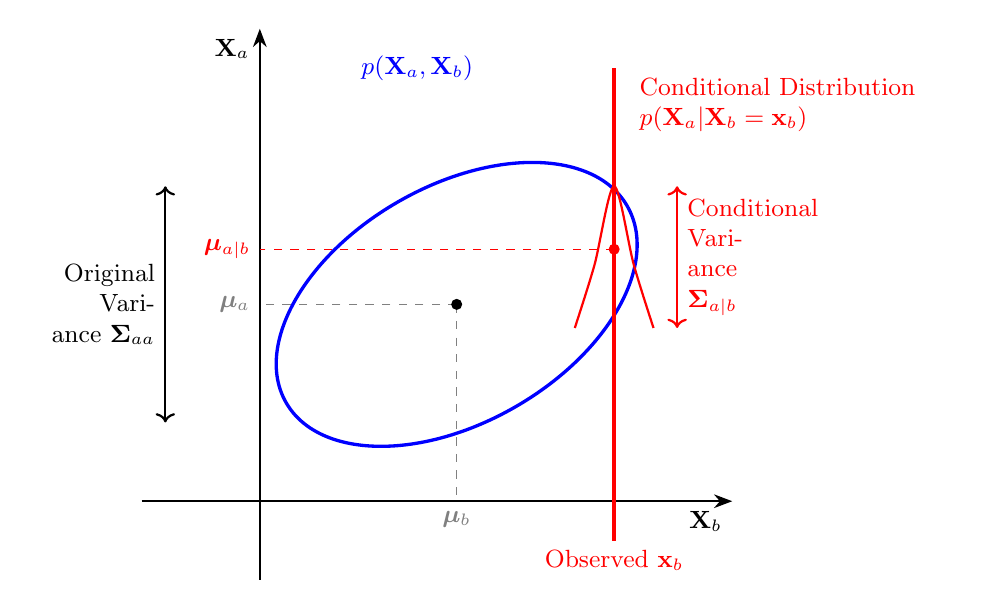
\begin{tikzpicture}[
        font=\sffamily,
        every node/.style={font=\small},
        arrow/.style={-Stealth, thick}
    ]
    % Axes
    \draw[-Stealth, thick] (-1.5,0) -- (6,0) node[below left] {$\vect{X}_b$};
    \draw[-Stealth, thick] (0,-1) -- (0,6) node[below left] {$\vect{X}_a$};

    % Joint Distribution Ellipse (representing a contour of p(Xa, Xb))
    \draw[blue, very thick, rotate around={30:(2.5,2.5)}] (2.5,2.5) ellipse (2.5cm and 1.5cm);
    \node[blue] at (2, 5.5) {$p(\vect{X}_a, \vect{X}_b)$};

    % Unconditional Means
    \draw[dashed, gray] (2.5,2.5) -- (2.5,0) node[below] {$\boldsymbol{\mu}_b$};
    \draw[dashed, gray] (2.5,2.5) -- (0,2.5) node[left] {$\boldsymbol{\mu}_a$};
    \fill[black] (2.5,2.5) circle (2pt);

    % Observation (the slice)
    \def\obsval{4.5}
    \draw[red, very thick] (\obsval, -0.5) -- (\obsval, 5.5);
    \node[red, below] at (\obsval, -0.5) {Observed $\vect{x}_b$};

    % Conditional Distribution p(Xa | Xb)
    \coordinate (slice_center) at (\obsval, 3.2); % Approximate center of the slice
    
    % Draw the 1D Gaussian bell curve for the conditional distribution
    \draw[red, thick, smooth] plot[domain=-1.5:1.5, samples=50] 
        coordinates {(\obsval-0.5, 3.2-1.0) (\obsval-0.25, 3.2-0.2) (\obsval, 3.2+0.8) (\obsval+0.25, 3.2-0.2) (\obsval+0.5, 3.2-1.0)};
    
    % Conditional Mean
    \draw[dashed, red] (slice_center) -- (0, 3.2) node[left] {$\boldsymbol{\mu}_{a|b}$};
    \fill[red] (slice_center) circle (2pt);
    
    % MODIFIED: Moved "Conditional Distribution..." text to be anchored to the left, just after the red line.
    \node[red, text width=4cm, align=left, anchor=north west] at (\obsval+0.2, 5.5)
        {Conditional Distribution $p(\vect{X}_a | \vect{X}_b=\vect{x}_b)$};

    % Illustrate variance reduction
    \draw[<->, thick, black] (-1.2, 1) -- (-1.2, 4) node[midway, left, text width=1.5cm, align=right] {Original Variance $\boldsymbol{\Sigma}_{aa}$};
    \draw[<->, thick, red] (\obsval+0.8, 2.2) -- (\obsval+0.8, 4.0) node[midway, right, text width=1cm] {Conditional Variance $\boldsymbol{\Sigma}_{a|b}$};

    \end{tikzpicture}%
}

\ifdefined\ispartofbook
  % This part is intentionally left blank when included in the main book.
\else
  % This part is for standalone compilation of the image.
  \conditionalgaussiandiagram
  \end{document}
\fi
 % Include the conditional Gaussian diagram

This chapter builds upon the one-dimensional statistical concepts from Chapter 1 and extends the analysis to the more complex and realistic multivariate setting. It will provide a comprehensive treatment of the "forward problem": the challenge of calculating the mean vector and full covariance matrix of a rectified multivariate normal (RMVN) distribution. The chapter will dissect the analytical and computational challenges that arise from inter-variable correlations, moving from a concrete 2D example to the general N-dimensional case and surveying the state-of-the-art methods for finding a solution.

\section{The Multivariate Normal Distribution: Parameter Estimation}
\label{sec:mvn_estimation}

The natural starting point for any multivariate analysis is the Multivariate Normal (MVN) distribution, also known as the multivariate Gaussian. It is the generalization of the familiar one-dimensional normal distribution to higher dimensions and serves as the fundamental building block for the models in this chapter \cite{Bishop2006PatternRecognition}.

An $N$-dimensional random vector $\vect{X}$ is said to have an MVN distribution if every linear combination of its components has a univariate normal distribution. It is completely characterized by two parameters: an $N \times 1$ mean vector $\boldsymbol{\mu}$ and an $N \times N$ covariance matrix $\boldsymbol{\Sigma}$. We denote this as $\vect{X} \sim \mathcal{N}(\boldsymbol{\mu}, \boldsymbol{\Sigma})$.

The focus of this section is on how these parameters are obtained from data. The standard approach is \textbf{Maximum Likelihood Estimation (MLE)}. Given a dataset of $m$ observations $\{\vect{x}_1, \dots, \vect{x}_m\}$, the principle of MLE is to find the parameter values $(\boldsymbol{\mu}, \boldsymbol{\Sigma})$ that maximize the probability of observing the given data. For the MVN distribution, this optimization yields a simple and intuitive closed-form solution \cite{Murphy2012ML}:
\begin{itemize}
    \item The MLE for the \textbf{mean vector} is the sample mean:
    \begin{equation}
        \hat{\boldsymbol{\mu}} = \frac{1}{m} \sum_{i=1}^m \vect{x}_i
    \end{equation}
    \item The MLE for the \textbf{covariance matrix} is the sample covariance:
    \begin{equation}
        \hat{\boldsymbol{\Sigma}} = \frac{1}{m} \sum_{i=1}^m (\vect{x}_i - \hat{\boldsymbol{\mu}})(\vect{x}_i - \hat{\boldsymbol{\mu}})^T
    \end{equation}
\end{itemize}
In practice, the unbiased estimator for the sample covariance, which uses a $\frac{1}{m-1}$ denominator, is often preferred. This process of fitting a Gaussian model to data is the first step in many statistical analysis pipelines.

\section{Properties of the MVN: Linearity, Marginals, and Conditionals}
\label{sec:mvn_properties}

The MVN distribution possesses several elegant properties that make it exceptionally tractable for analytical work.
\begin{itemize}
    \item \textbf{Closure under Affine Transformations:} The MVN family is closed under affine transformations. If $\vect{X} \sim \mathcal{N}(\boldsymbol{\mu}, \boldsymbol{\Sigma})$, then any linear transformation of that vector, $\vect{Y} = \matr{A}\vect{X} + \vect{b}$, is also normally distributed with mean $\matr{A}\boldsymbol{\mu} + \vect{b}$ and covariance $\matr{A}\boldsymbol{\Sigma}\matr{A}^T$. This property is fundamental to the analysis of linear layers in neural networks.

    \item \textbf{Marginal Distributions:} Any subset of a multivariate normal vector is also multivariate normal. If we partition a vector $\vect{X} = [\vect{X}_a^T, \vect{X}_b^T]^T$, the marginal distribution of $\vect{X}_a$ is simply $\mathcal{N}(\boldsymbol{\mu}_a, \boldsymbol{\Sigma}_{aa})$, where $\boldsymbol{\mu}_a$ and $\boldsymbol{\Sigma}_{aa}$ are the corresponding blocks of the original mean vector and covariance matrix.

    \item \textbf{Conditional Distributions:} Crucially, the conditional distribution of one subset given another is also Gaussian. The conditional distribution $p(\vect{X}_a | \vect{X}_b)$ is normal with a conditional mean and covariance given by:
    \begin{align}
        \boldsymbol{\mu}_{a|b} &= \boldsymbol{\mu}_a + \boldsymbol{\Sigma}_{ab} \boldsymbol{\Sigma}_{bb}^{-1} (\vect{X}_b - \boldsymbol{\mu}_b) \\
        \boldsymbol{\Sigma}_{a|b} &= \boldsymbol{\Sigma}_{aa} - \boldsymbol{\Sigma}_{ab} \boldsymbol{\Sigma}_{bb}^{-1} \boldsymbol{\Sigma}_{ba}
    \end{align}
    These formulas are the engine of statistical inference in Gaussian models. The conditional mean provides the best linear estimate of $\vect{X}_a$ given $\vect{X}_b$, and the conditional covariance quantifies the remaining uncertainty. These equations form the basis for many generative models and analytical frameworks \cite{Murphy2012ML}.
\end{itemize}

\begin{figure}[h!]
    \centering
    \scalebox{0.8}{\conditionalgaussiandiagram}
    \caption{An illustration of conditioning a bivariate normal distribution. Observing a value for $\vect{X}_b$ is equivalent to taking a slice through the joint distribution. The resulting conditional distribution $p(\vect{X}_a | \vect{X}_b)$ is a new Gaussian with an updated mean ($\boldsymbol{\mu}_{a|b}$) and a reduced variance ($\boldsymbol{\Sigma}_{a|b}$).}
    \label{fig:conditional_gaussian}
\end{figure}

\section{Defining the Rectified Multivariate Normal Distribution (RMVN)}
\label{sec:define_rmvn}

The Rectified Multivariate Normal (RMVN) distribution is the result of applying the element-wise rectification operator to a vector drawn from an MVN distribution: $\vect{Y} = \max(\vect{0}, \vect{X})$ where $\vect{X} \sim \mathcal{N}(\boldsymbol{\mu}, \boldsymbol{\Sigma})$.

This operation induces a combinatorial explosion in the underlying structure of the problem. While the one-dimensional space $\mathbb{R}$ is partitioned into two regions by the rectifier, the $N$-dimensional space $\mathbb{R}^N$ is partitioned into $2^N$ orthants, each defined by a unique combination of signs of the components of $\vect{X}$. The rectification operator maps each of these $2^N$ orthants onto a distinct subspace within the non-negative orthant $\mathbb{R}^N_+$.

Consequently, the resulting distribution of $\vect{Y}$ is no longer a simple two-part mixture. It becomes a complex mixture of $2^N$ components:
\begin{itemize}
    \item One fully continuous distribution on the interior of $\mathbb{R}^N_+$ (where all components are positive), which is an N-dimensional Truncated Multivariate Normal (TMVN) distribution.
    \item $2^N-1$ distributions supported on the lower-dimensional faces, edges, and vertices of this orthant (where one or more components are exactly zero). The most extreme case collapses the entire negative orthant to a single point mass at the origin, $\vect{Y} = \vect{0}$.
\end{itemize}
This fundamental change elevates the problem from a tractable statistical exercise to a formidable computational and analytical endeavor.

\section{The Forward Problem: Moments of the RMVN}
\label{sec:forward_problem_rmvn}

The forward problem is to calculate the first two moments of the rectified vector $\mathbf{Y} = \max(\mathbf{0}, \mathbf{X})$—the rectified mean vector, $\boldsymbol{\mu}_Y = \E[\mathbf{Y}]$, and the rectified covariance matrix, $\boldsymbol{\Sigma}_Y = \text{Cov}(\mathbf{Y})$—given the original parameters $(\boldsymbol{\mu}, \boldsymbol{\Sigma})$.

This task is fundamentally dependent on computing moments of the \textbf{Truncated Multivariate Normal (TMVN)} distribution. The $(i, j)$-th element of the second raw moment matrix is $E[Y_i Y_j] = E[\max(0, X_i)\max(0, X_j)]$. The integrand for this expectation is non-zero only when both $x_i > 0$ and $x_j > 0$. Therefore, the integral is:
\begin{equation}
E[Y_i Y_j] = \int_{x_i > 0, x_j > 0} x_i x_j f(\mathbf{x}; \boldsymbol{\mu}, \boldsymbol{\Sigma}) d\mathbf{x}
\end{equation}
This integral is the un-normalized second cross-moment of the original MVN truncated to the region where $x_i > 0$ and $x_j > 0$. The correlation structure encoded in $\boldsymbol{\Sigma}$ prevents this N-dimensional integral from decomposing into simpler 1D integrals. For dimensions $N > 2$, this integral, and thus the rectified moments, lack a general closed-form solution and are considered analytically intractable.

\section{A Concrete Example: The Bivariate (2D) Case}
\label{sec:bivariate_case}

The bivariate case ($N=2$) is the highest dimension for which reasonably explicit analytical formulas can be presented. The problem is to find the five rectified moments from the five original parameters $(\mu_1, \mu_2, \sigma_1, \sigma_2, \rho)$. The rectified means and variances depend only on the marginal distributions and are identical in form to the 1D case. The primary challenge is the rectified covariance, $\text{Cov}(Y_1, Y_2) = E[Y_1 Y_2] - E[Y_1]E[Y_2]$. The expectation of the product, $E[Y_1 Y_2]$, is given by the integral of $x_1 x_2$ over the positive quadrant of the bivariate normal distribution.

The analytical expression for this moment is well-established in the statistical literature \cite{Muthen1990CensoredMoments}. The complete expression for $E[Y_1 Y_2]$ is:
\begin{align}
E[Y_1 Y_2] = & (\mu_1 \mu_2 + \rho \sigma_1 \sigma_2) \Phi_2\left(\frac{\mu_1}{\sigma_1}, \frac{\mu_2}{\sigma_2}; \rho\right) \nonumber \\
& + \mu_1 \sigma_2 \phi\left(\frac{\mu_2}{\sigma_2}\right)\Phi\left(\frac{\mu_1/\sigma_1 - \rho \mu_2/\sigma_2}{\sqrt{1-\rho^2}}\right) \nonumber \\
& + \mu_2 \sigma_1 \phi\left(\frac{\mu_1}{\sigma_1}\right)\Phi\left(\frac{\mu_2/\sigma_2 - \rho \mu_1/\sigma_1}{\sqrt{1-\rho^2}}\right) \nonumber \\
& + \sigma_1 \sigma_2 \sqrt{1-\rho^2} \phi_2\left(\frac{\mu_1}{\sigma_1}, \frac{\mu_2}{\sigma_2}; \rho\right)
\end{align}
where $\phi_2$ and $\Phi_2$ are the PDF and CDF of the standard bivariate normal distribution. This formula explicitly demonstrates the complex dependence on all five original parameters and the reliance on the bivariate normal CDF, which itself must be computed numerically.

\section{Computational Methodologies for High Dimensions}
\label{sec:computational_methods}

Given the analytical intractability of the RMVN moments in high dimensions, the focus of modern research has been on developing effective computational algorithms.
\begin{enumerate}
    \item \textbf{The Moment Generating Function (MGF) Approach:} A classical approach pioneered by Tallis (1961) involves differentiating the MGF of the truncated distribution \cite{Tallis1961MGF}. While theoretically sound, the MGF itself is a complex integral, and differentiating it becomes exceptionally "tedious" and computationally explosive, making it impractical for high dimensions.

    \item \textbf{Recurrence Relation Algorithms:} The state-of-the-art approach for high-precision numerical computation involves the use of recurrence relations \cite{KanRobotti2017TruncatedMoments}. This methodology transforms the problem from direct, intractable integration into a computationally feasible recursive procedure. It expresses a high-dimensional integral in terms of a sum of simpler, lower-dimensional integrals, which can be computed efficiently.

    \item \textbf{Monte Carlo Methods:} When analytical precision is not paramount, Monte Carlo methods provide a flexible alternative.
    \begin{itemize}
        \item \textbf{Direct Simulation:} The simplest method is to draw a large number of samples from the original MVN, apply the rectifier to each sample, and then compute the sample moments of the resulting set.
        \item \textbf{Gibbs Sampling:} A more sophisticated Markov Chain Monte Carlo (MCMC) technique, Gibbs sampling is particularly well-suited for sampling from truncated multivariate distributions. It iteratively draws from the conditional distribution of each variable given the others, which is a simple truncated univariate normal \cite{Geweke1991Gibbs}.
    \end{itemize}
\end{enumerate}

\ifdefined\ispartofbook
\else
  \begin{thebibliography}{99}

\bibitem{AdadiBerrada2018XAISurvey}
Adadi, A., \& Berrada, M. (2018). Peeking Inside the Black-Box: A Survey on Explainable Artificial Intelligence (XAI). \textit{IEEE Access}.

\bibitem{AlainBengio2016Probes}
Alain, G., \& Bengio, Y. (2016). Understanding intermediate layers using linear classifier probes. \textit{arXiv preprint arXiv:1610.01644}.

\bibitem{Amemiya1985Econometrics}
Amemiya, T. (1985). \textit{Advanced Econometrics}. Harvard University Press.

\bibitem{Arora2025ReLUOutputDist}
Arora, R., Basu, A., Mianjy, P., \& Mukherjee, A. (2025). On the Exact Computation of the Output Distribution of a ReLU Network. \textit{arXiv preprint arXiv:2503.22082}.

\bibitem{BarrSherrill1999TruncatedNormal}
Barr, D. R., \& Sherrill, E. T. (1999). Mean and variance of truncated normal distributions. \textit{The American Statistician, 53}(4), 357-361.

\bibitem{Bishop2006PatternRecognition}
Bishop, C. M. (2006). \textit{Pattern Recognition and Machine Learning}. Springer.

\bibitem{Bottou2018Optimization}
Bottou, L., Curtis, F. E., \& Nocedal, J. (2018). Optimization methods for large-scale machine learning. \textit{SIAM Review}, 60(2), 223-311.

\bibitem{ChoSaul2014RectifiedGaussian}
Cho, K., \& Saul, L. K. (2014). On the properties of the rectified Gaussian distribution. \textit{arXiv preprint arXiv:1406.4533}.

\bibitem{DansbeckerRELUKaggle}
Dansbecker, M. (n.d.). \textit{Rectified Linear Units (ReLU) in Deep Learning}. Kaggle. Retrieved July 23, 2025, from \url{https://www.kaggle.com/code/dansbecker/rectified-linear-units-relu-in-deep-learning}

\bibitem{Ding2013RectifiedFactor}
Ding, Z., He, Z., \& Carin, L. (2013). Rectified factor networks. In \textit{Advances in Neural Information Processing Systems 26} (pp. 1106-1114).

\bibitem{FreyHinton1999Transformations}
Frey, B. J., \& Hinton, G. E. (1999). Variational learning in nonlinear Gaussian belief networks. \textit{Neural Computation}, 11(1), 193-213.

\bibitem{Fukushima1980Neocognitron}
Fukushima, K. (1980). Neocognitron: A self-organizing neural network model for a mechanism of pattern recognition unaffected by shift in position. \textit{Biological Cybernetics}, 36(4), 193-202.

\bibitem{GalGhahramani2016DropoutBayes}
Gal, Y., \& Ghahramani, Z. (2016). Dropout as a Bayesian approximation: Representing model uncertainty in deep learning. In \textit{International conference on machine learning} (pp. 1050-1059).

\bibitem{Genz2009Computation}
Genz, A., \& Bretz, F. (2009). \textit{Computation of multivariate normal and t probabilities}. Springer Science \& Business Media.

\bibitem{Geweke1991Gibbs}
Geweke, J. (1991). Efficient simulation from the multivariate normal and Student-t distributions subject to linear constraints. In \textit{Computing Science and Statistics: Proceedings of the 23rd Symposium on the Interface} (pp. 571-578).

\bibitem{GlorotBordesBengio2011DeepSparse}
Glorot, X., Bordes, A., \& Bengio, Y. (2011). Deep sparse rectifier neural networks. In \textit{Proceedings of the fourteenth international conference on artificial intelligence and statistics} (pp. 315-323).

\bibitem{GlorotBengio2010Difficulty}
Glorot, X., \& Bengio, Y. (2010). Understanding the difficulty of training deep feedforward neural networks. In \textit{Proceedings of the thirteenth international conference on artificial intelligence and statistics} (pp. 249-256).

\bibitem{Goodfellow2016Book}
Goodfellow, I., Bengio, Y., \& Courville, A. (2016). \textit{Deep Learning}. MIT Press.

\bibitem{HaninRolnick2019ActivationPatterns}
Hanin, B., \& Rolnick, D. (2019). Deep ReLU Networks Have Surprisingly Few Activation Patterns. \textit{Advances in Neural Information Processing Systems}.

\bibitem{He2015Delving}
He, K., Zhang, X., Ren, S., \& Sun, J. (2015). Delving deep into rectifiers: Surpassing human-level performance on imagenet classification. In \textit{Proceedings of the IEEE international conference on computer vision} (pp. 1026-1034).

\bibitem{Hochreiter2001GradientFlow}
Hochreiter, S., Bengio, Y., Frasconi, P., \& Schmidhuber, J. (2001). \textit{Gradient flow in recurrent nets: the difficulty of learning long-term dependencies}. In A field guide to dynamical recurrent networks. IEEE Press.

\bibitem{Hornik1989UniversalApprox}
Hornik, K., Stinchcombe, M., \& White, H. (1989). \textit{Multilayer feedforward networks are universal approximators}. Neural Networks, 2(5), 359-366.

\bibitem{KanRobotti2017TruncatedMoments}
Kan, R., \& Robotti, C. (2017). On the moments of folded and truncated multivariate normal distributions. \textit{Journal of Computational and Graphical Statistics, 26}(4), 930-934.

\bibitem{KingmaBa2014Adam}
Kingma, D. P., \& Ba, J. (2014). Adam: A method for stochastic optimization. \textit{arXiv preprint arXiv:1412.6980}.

\bibitem{LeCun1998MNIST}
LeCun, Y., Bottou, L., Bengio, Y., \& Haffner, P. (1998). Gradient-based learning applied to document recognition. \textit{Proceedings of the IEEE}, 86(11), 2278-2324.

\bibitem{LeCun2012EfficientBackprop}
LeCun, Y., Bottou, L., Orr, G. B., \& Müller, K. R. (2012). Efficient backprop. In \textit{Neural networks: Tricks of the trade} (pp. 9-48). Springer.

\bibitem{Liu2022RectifiedFlow}
Liu, X., Gong, C., \& Liu, Q. (2022). Rectified flow: A marginal preserving approach to optimal transport. \textit{arXiv preprint arXiv:2209.14577}.

\bibitem{LundbergLee2017SHAP}
Lundberg, S. M., \& Lee, S. I. (2017). A unified approach to interpreting model predictions. In \textit{Advances in neural information processing systems} (pp. 4765-4774).

\bibitem{Mazur2015BackpropExample}
Mazur, M. (2015). A Step by Step Backpropagation Example. \textit{Matt Mazur blog}. Retrieved August 7, 2025, from \url{https://mattmazur.com/2015/03/17/a-step-by-step-backpropagation-example/}

\bibitem{Murphy2012ML}
Murphy, K. P. (2012). \textit{Machine Learning: A Probabilistic Perspective}. MIT Press.

\bibitem{Muthen1990CensoredMoments}
Muthén, B. (1990). \textit{Moments of the censored and truncated bivariate normal distribution}. British Journal of Mathematical and Statistical Psychology, 43(1), 131-143.

\bibitem{NairHinton2010ReLU}
Nair, V., \& Hinton, G. E. (2010). Rectified linear units improve restricted boltzmann machines. In \textit{Proceedings of the 27th international conference on machine learning (ICML-10)} (pp. 807-814).

\bibitem{Nielsen2015Book}
Nielsen, M. A. (2015). \textit{Neural networks and deep learning}. Determination press.

\bibitem{Pinkus1999ApproximationTheory}
Pinkus, A. (1999). \textit{Approximation theory of the MLP model in neural networks}. Acta Numerica, 8, 143-195.

\bibitem{Poole2016ExponentialExpressivity}
Poole, B., Lahiri, S., Raghu, M., Sohl-Dickstein, J., \& Ganguli, S. (2016). Exponential expressivity in deep neural networks through transient chaos. \textit{Advances in neural information processing systems}, 29.

\bibitem{Ribeiro2016LIME}
Ribeiro, M. T., Singh, S., \& Guestrin, C. (2016). "Why Should I Trust You?": Explaining the Predictions of Any Classifier. \textit{Proceedings of the 22nd ACM SIGKDD International Conference on Knowledge Discovery and Data Mining}.

\bibitem{Rudin2019StopExplaining}
Rudin, C. (2019). Stop explaining black box machine learning models for high stakes decisions and use interpretable models instead. \textit{Nature Machine Intelligence}, 1(5), 206-215.

\bibitem{Rumelhart1986Backprop}
Rumelhart, D. E., Hinton, G. E., \& Williams, R. J. (1986). Learning representations by back-propagating errors. \textit{Nature}, 323(6088), 533-536.

\bibitem{Schiendorfer2020BackpropExample}
Schiendorfer, A. (2020). A worked example of backpropagation. \textit{Connecting deep dots blog}. Retrieved August 7, 2025, from \url{https://alexander-schiendorfer.github.io/2020/02/24/a-worked-example-of-backprop.html}

\bibitem{Schoenholz2017DeepInfoProp}
Schoenholz, S. S., Gilmer, J., Ganguli, S., \& Sohl-Dickstein, J. (2017). Deep information propagation. \textit{arXiv preprint arXiv:1611.01232}.

\bibitem{Selvaraju2017GradCAM}
Selvaraju, R. R., Cogswell, M., Das, A., Vedantam, R., Parikh, D., \& Batra, D. (2017). Grad-cam: Visual explanations from deep networks via gradient-based localization. In \textit{Proceedings of the IEEE international conference on computer vision} (pp. 618-626).

\bibitem{Socci1998RectifiedGaussian}
Socci, N. D., Lee, D. D., \& Seung, H. S. (1998). The rectified gaussian distribution. In \textit{Advances in Neural Information Processing Systems} (pp. 350-356).

\bibitem{Tallis1961MGF}
Tallis, G. M. (1961). The moment generating function of the truncated multi-normal distribution. \textit{Journal of the Royal Statistical Society: Series B (Methodological)}, 23(1), 223-229.

\bibitem{Tobin1958LimitedDependent}
Tobin, J. (1958). \textit{Estimation of Relationships for Limited Dependent Variables}. Econometrica, 26(1), 24-36.

\bibitem{Wright2024AnalyticCovariance}
Wright, L., et al. (2024). An Analytic Solution to Covariance Propagation in Neural Networks. \textit{Proceedings of Machine Learning Research}.

\bibitem{Zayyani2016FastRectified}
Zayyani, H., Babaie-Zadeh, M., \& Jutten, C. (2016). Fast rectified sparse Bayesian learning. \textit{IEEE Transactions on Signal Processing}, 64(14), 3788-3799.

\end{thebibliography}

  \end{document}
\fi
